\section{Sequence Diagrams}

\subsection{General Sequence}
\begin{figure}[!htb]
    \centering
    \fbox{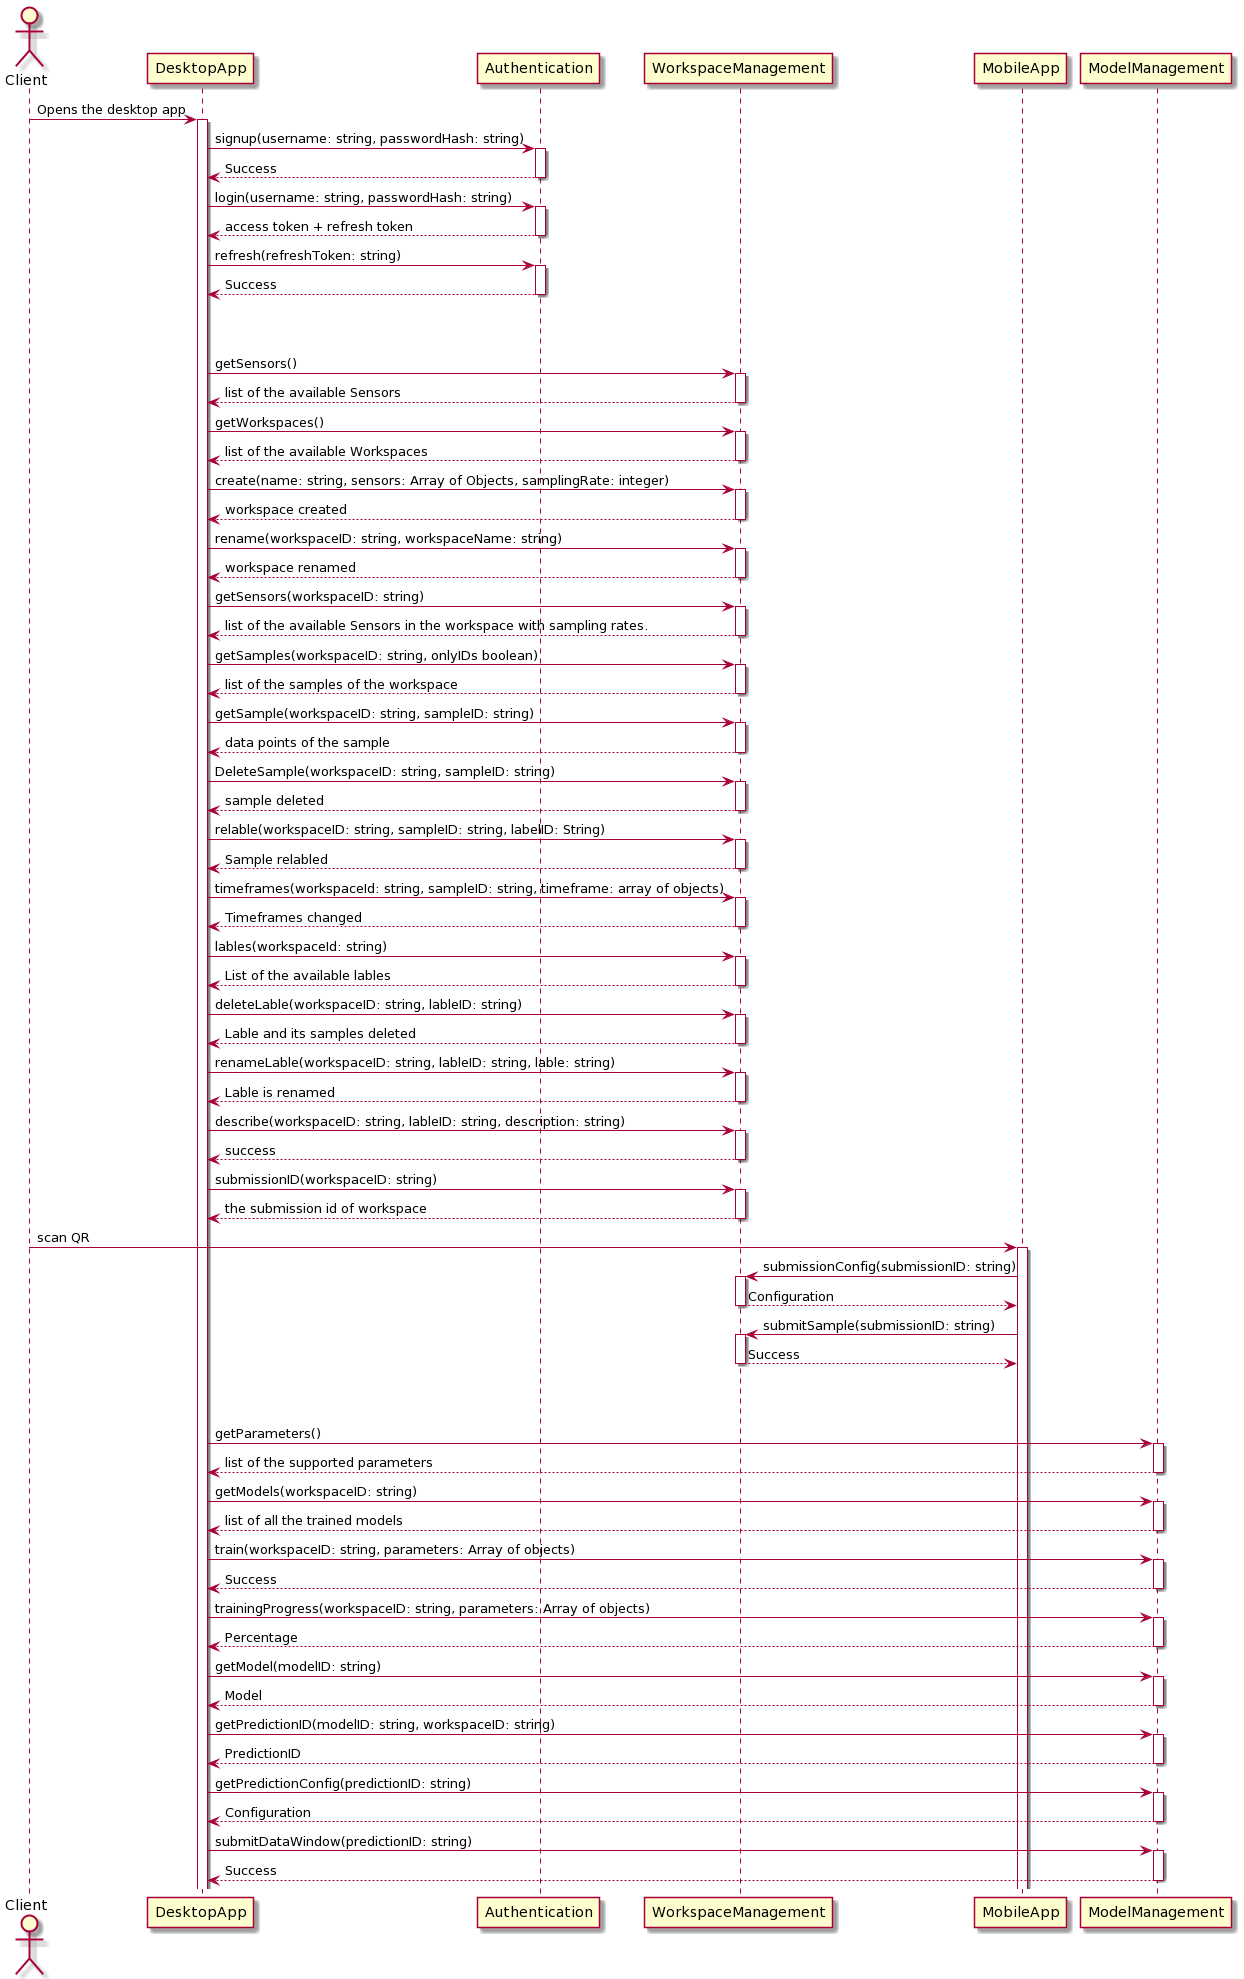
\includegraphics[width = .98\textwidth, height = .80\textheight]{figures/seq-general.png}}
    \caption{General Sequence}
    \label{fig:seq-general}
\end{figure}

\textbf{explanation}

\subsection{Desktop Client}

\subsubsection{Authentication}
\begin{figure}[hb]
    \centering
    \fbox{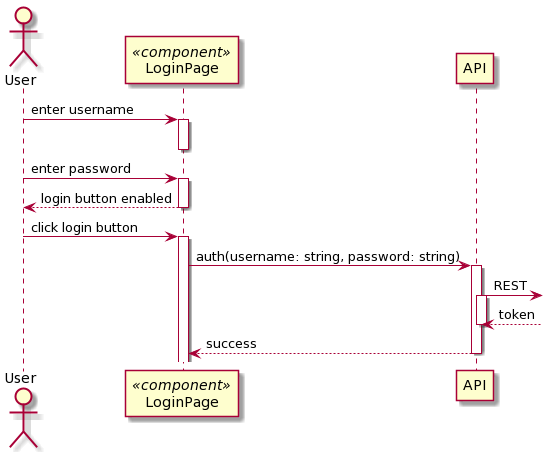
\includegraphics[width = .98\textwidth]{figures/seq-desktop-auth.png}}
    \caption{Authentication Sequence}
    \label{fig:seq-desktop-auth}
\end{figure}

\textbf{explanation}
\newpage

\subsubsection{Workspace Creation}
\begin{figure}[!htb]
    \centering
    \fbox{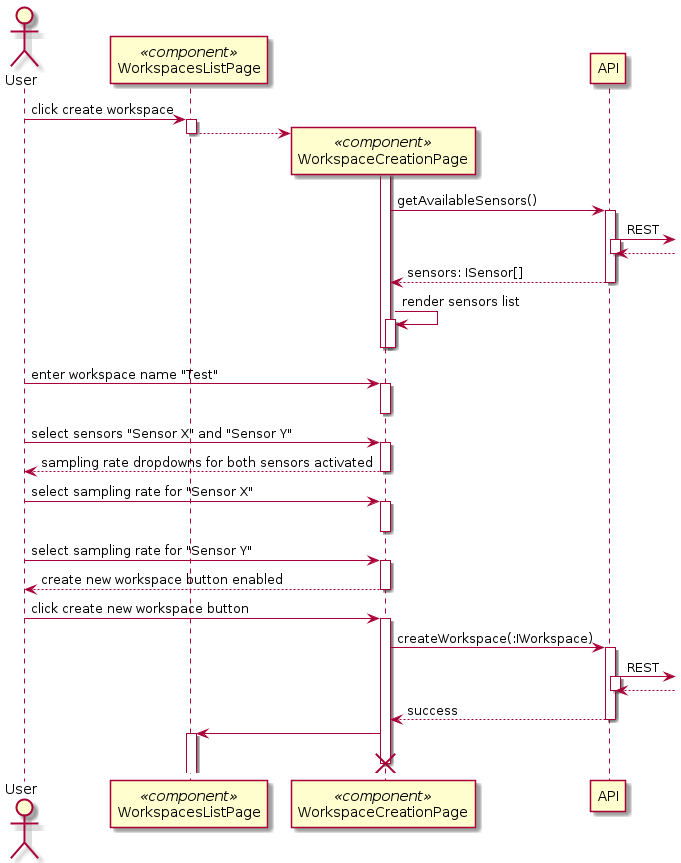
\includegraphics[width = .98\textwidth]{figures/seq-desktop-workspace-create.png}}
    \caption{Workspace Creation Sequence}
    \label{fig:seq-desktop-workspace-create}
\end{figure}

\textbf{explanation}
\newpage

\subsubsection{Fitting a Sample}
\begin{figure}[!htb]
    \centering
    \fbox{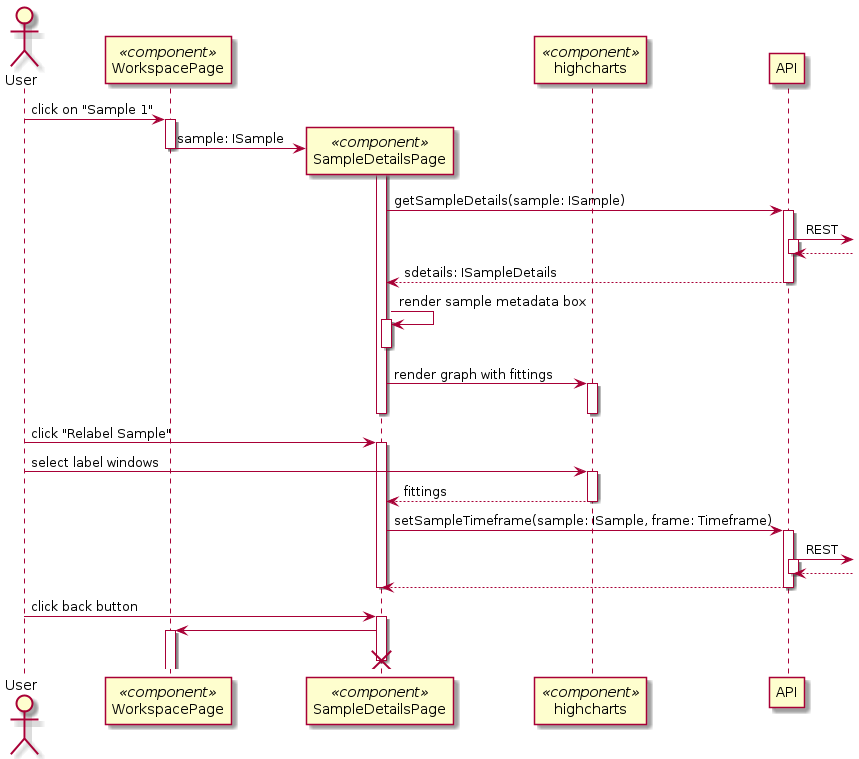
\includegraphics[width = .98\textwidth]{figures/seq-fitting-a-sample.png}}
    \caption{Sample Fitting Sequence}
    \label{fig:seq-fitting-a-sample}
\end{figure}

\textbf{explanation}
\newpage

\subsection{Mobile Client}

\subsection{Authentication}

This diagram shows the registration and validation process of new user accounts. The user first registers with his email, username and a password of his choice and then receives an email that has a validation code. The user enters this token to the desktop client and validates his account.
\subsubsection{Registration and Validation}
\begin{figure}[!htb]
    \centering
    \fbox{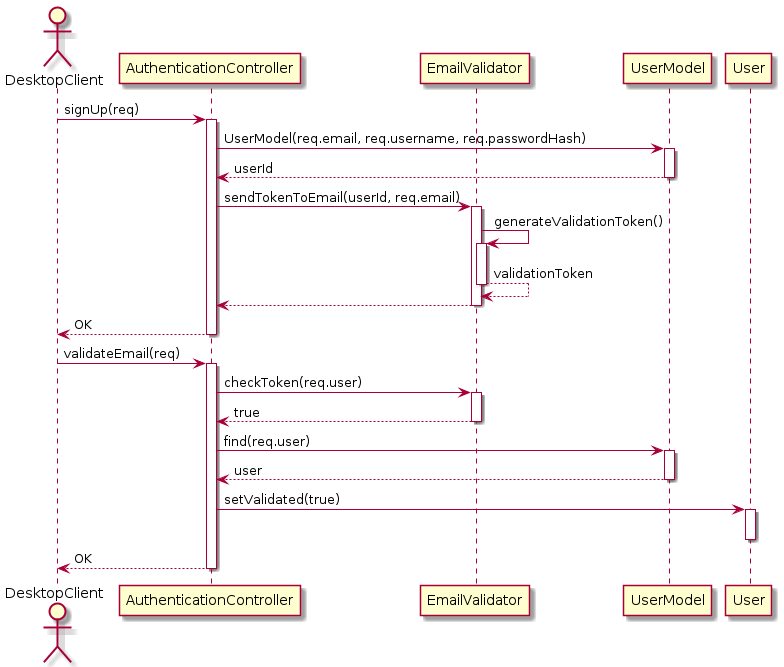
\includegraphics[width = 0.98\textwidth, height = 0.78\textheight]{figures/seq-auth-register-and-validate.png}}
    \caption{Registration and Validation}
    \label{fig:seq-auth-register-and-validate}
\end{figure}

\subsubsection{Login}
This diagram shows the login process. The user has already created an account and logs in. The received token is valid for a set amount of time which is then refresh by another token.
\begin{figure}[!htb]
    \centering
    \fbox{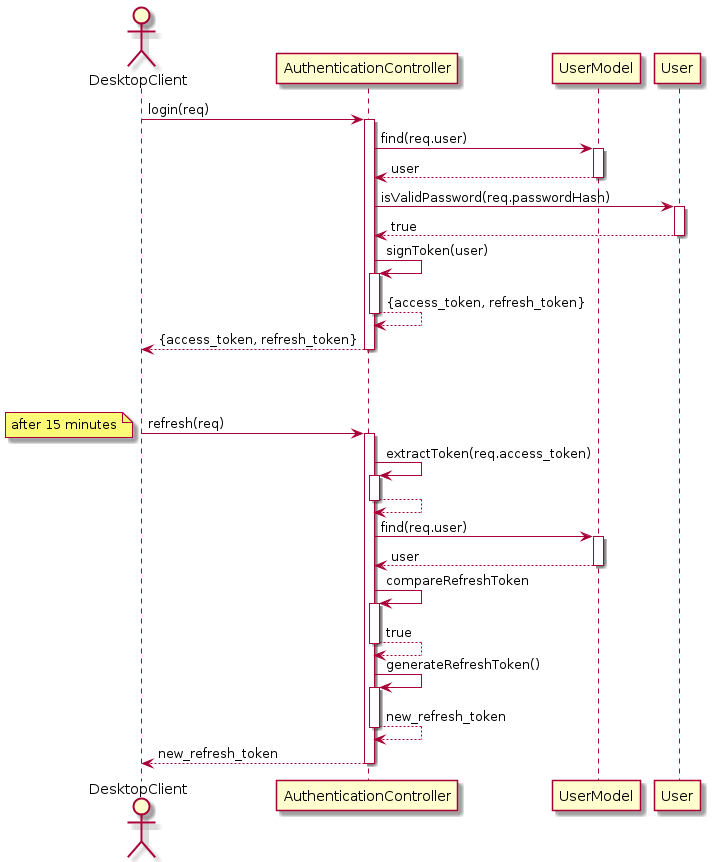
\includegraphics[width = 0.98\textwidth, height = 0.78\textheight]{figures/seq-auth-login.png}}
    \caption{Authentication Login}
    \label{fig:seq-auth-login}
\end{figure}

\subsection{Workspace Management}

\subsubsection{Create and Rename Workspace}
In this diagram, the user has no workspace initially. He then access the workspace creation tab of the desktop client. The desktop client asks the server which sensors are available as well as their default and maximum sampling rates. The user chooses the sensors he wishes to use and a name to his workspace. After creating it, the user renames the workspace.
\begin{figure}[!htb]
    \centering
    \fbox{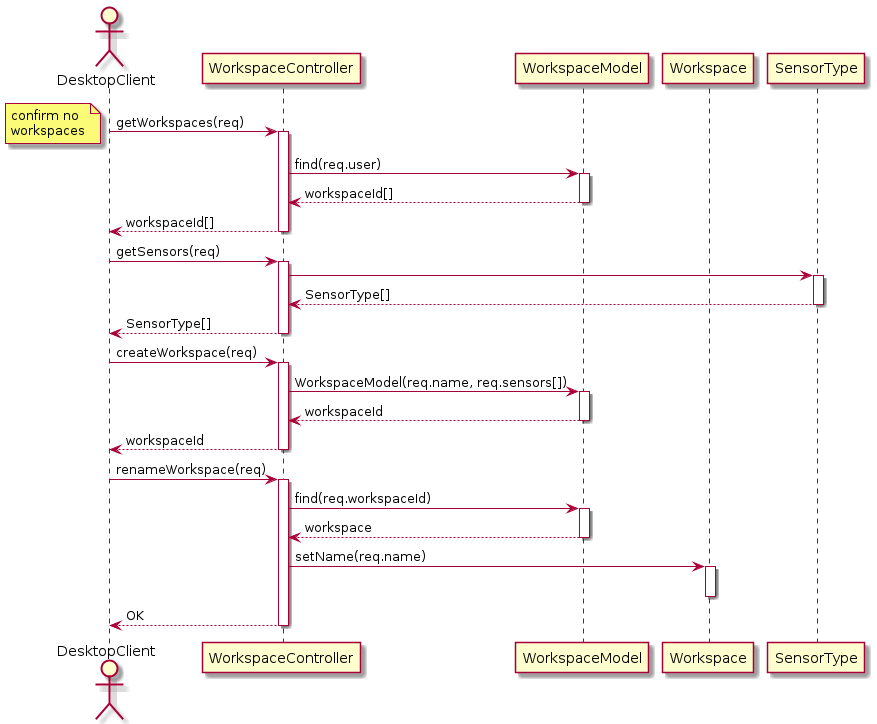
\includegraphics[width = 0.98\textwidth, height = 0.78\textheight]{figures/seq-workspace-create-and-rename.png}}
    \caption{Create and Rename}
    \label{fig:seq-workspace-create-and-rename}
\end{figure}
\newpage

\subsubsection{Submit Sample}
This diagram depicts the sample submission process. To start the sample collection, the desktop client asks for a submission id. After receiving the submission id, it embeds the id to a QR code which is scanned by the mobile client. The mobile client requests the submission config, i.e. which sensors are to be used for the recording and which labels are available. After the recording concludes, the sample is pushed to the server. A new entry for the sample is created in the server database.
\begin{figure}[!htb]
    \centering
    \fbox{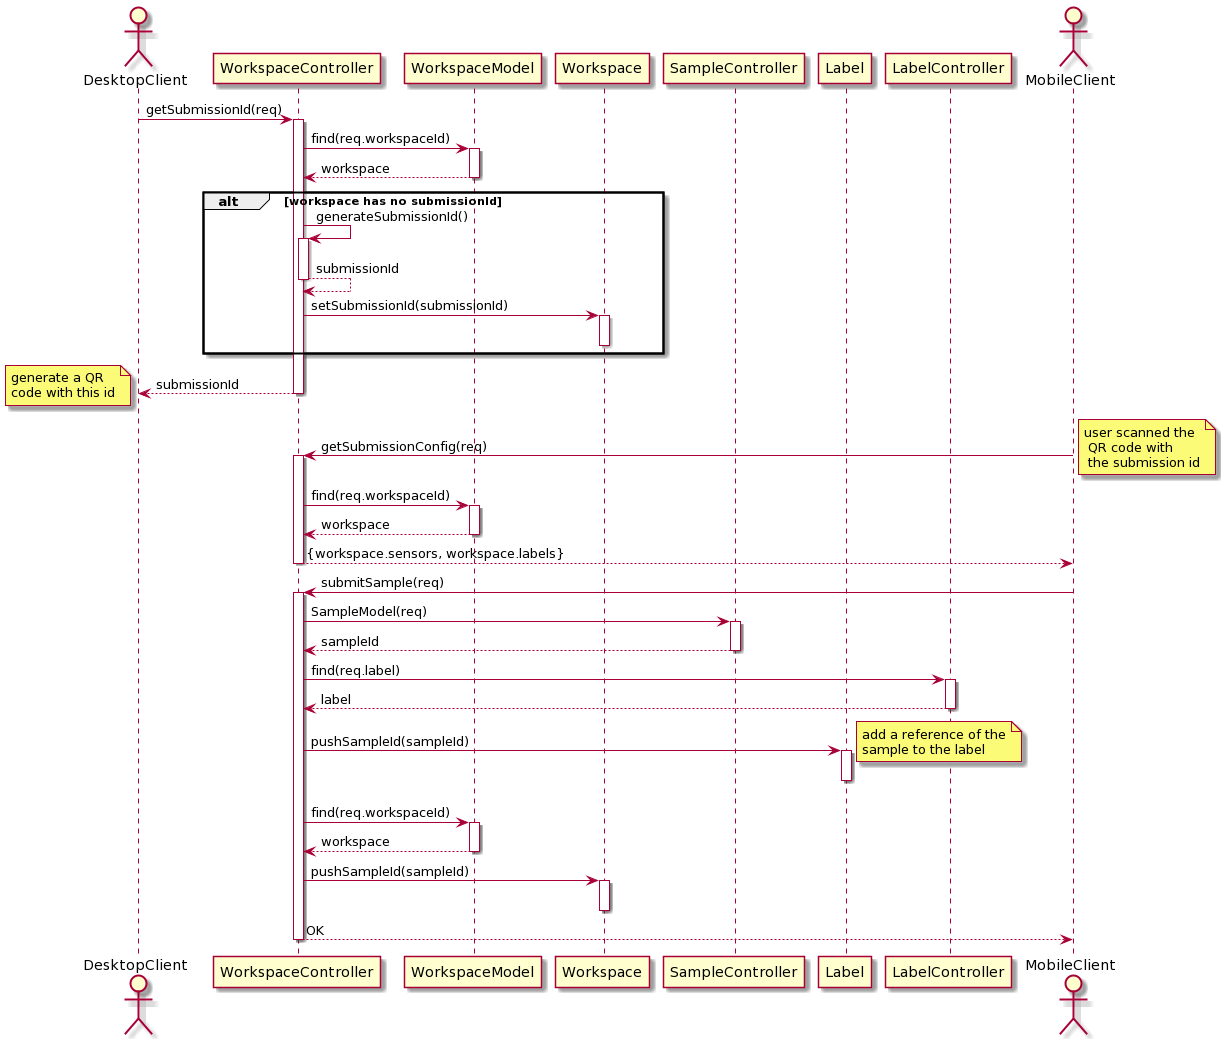
\includegraphics[width = 0.98\textwidth, height = 0.78\textheight]{figures/seq-workspace-submit-data.png}}
    \caption{Submit Data}
    \label{fig:seq-workspace-submit-data}
\end{figure}

\subsubsection{Create, Add Description and Delete Labels}
In this diagram, the user creates a new label to use for his samples by choosing a name. He then adds a description to the label. After that, he deletes a label from the workspace which in turn deletes all the samples in the workspace with that label.
\begin{figure}[!htb]
    \centering
    \fbox{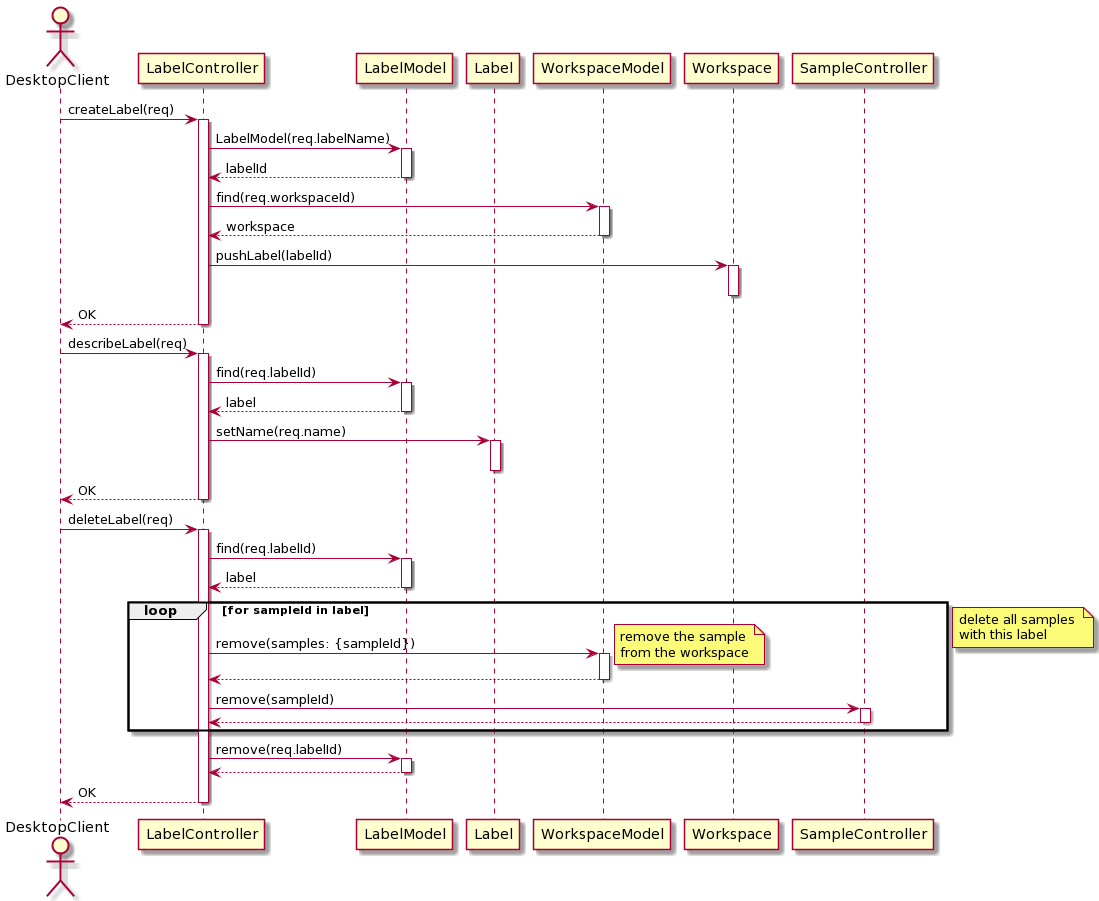
\includegraphics[width = 0.98\textwidth, height = 0.78\textheight]{figures/seq-workspace-management.png}}
    \caption{General Workspace Management}
    \label{fig:seq-workspace-management}
\end{figure}

\subsection{Model Management}

\subsubsection{Training a Model}
This sequence diagram shows how a train request is handled in the Model Management Server. In the beginning, a database connection is established, a Router instance is created, and a new workspace is created with the createModelWorkspace request from the Workspace Management Server.
The user first requests all the available training parameters with the getParameters request. Then the user requests training a model with the given name and training parameters. The model training is done in a Trainer instance. The training can be seen as a pipeline with the following parts: Retrieving samples, splitting to windows, imputation, feature extraction, normalization, classification and storing the new model in the database. The results of the steps from retrieving samples to feature extraction from recent model trainings are stored in the database, and they can be used if the samples or the parameters haven't changed. At the end, the created imputer, normalizer and classifier objects as well as its performance metrics are stored in the new MLModel instance and then stored in the database.
\begin{figure}[!htb]
    \centering
    \fbox{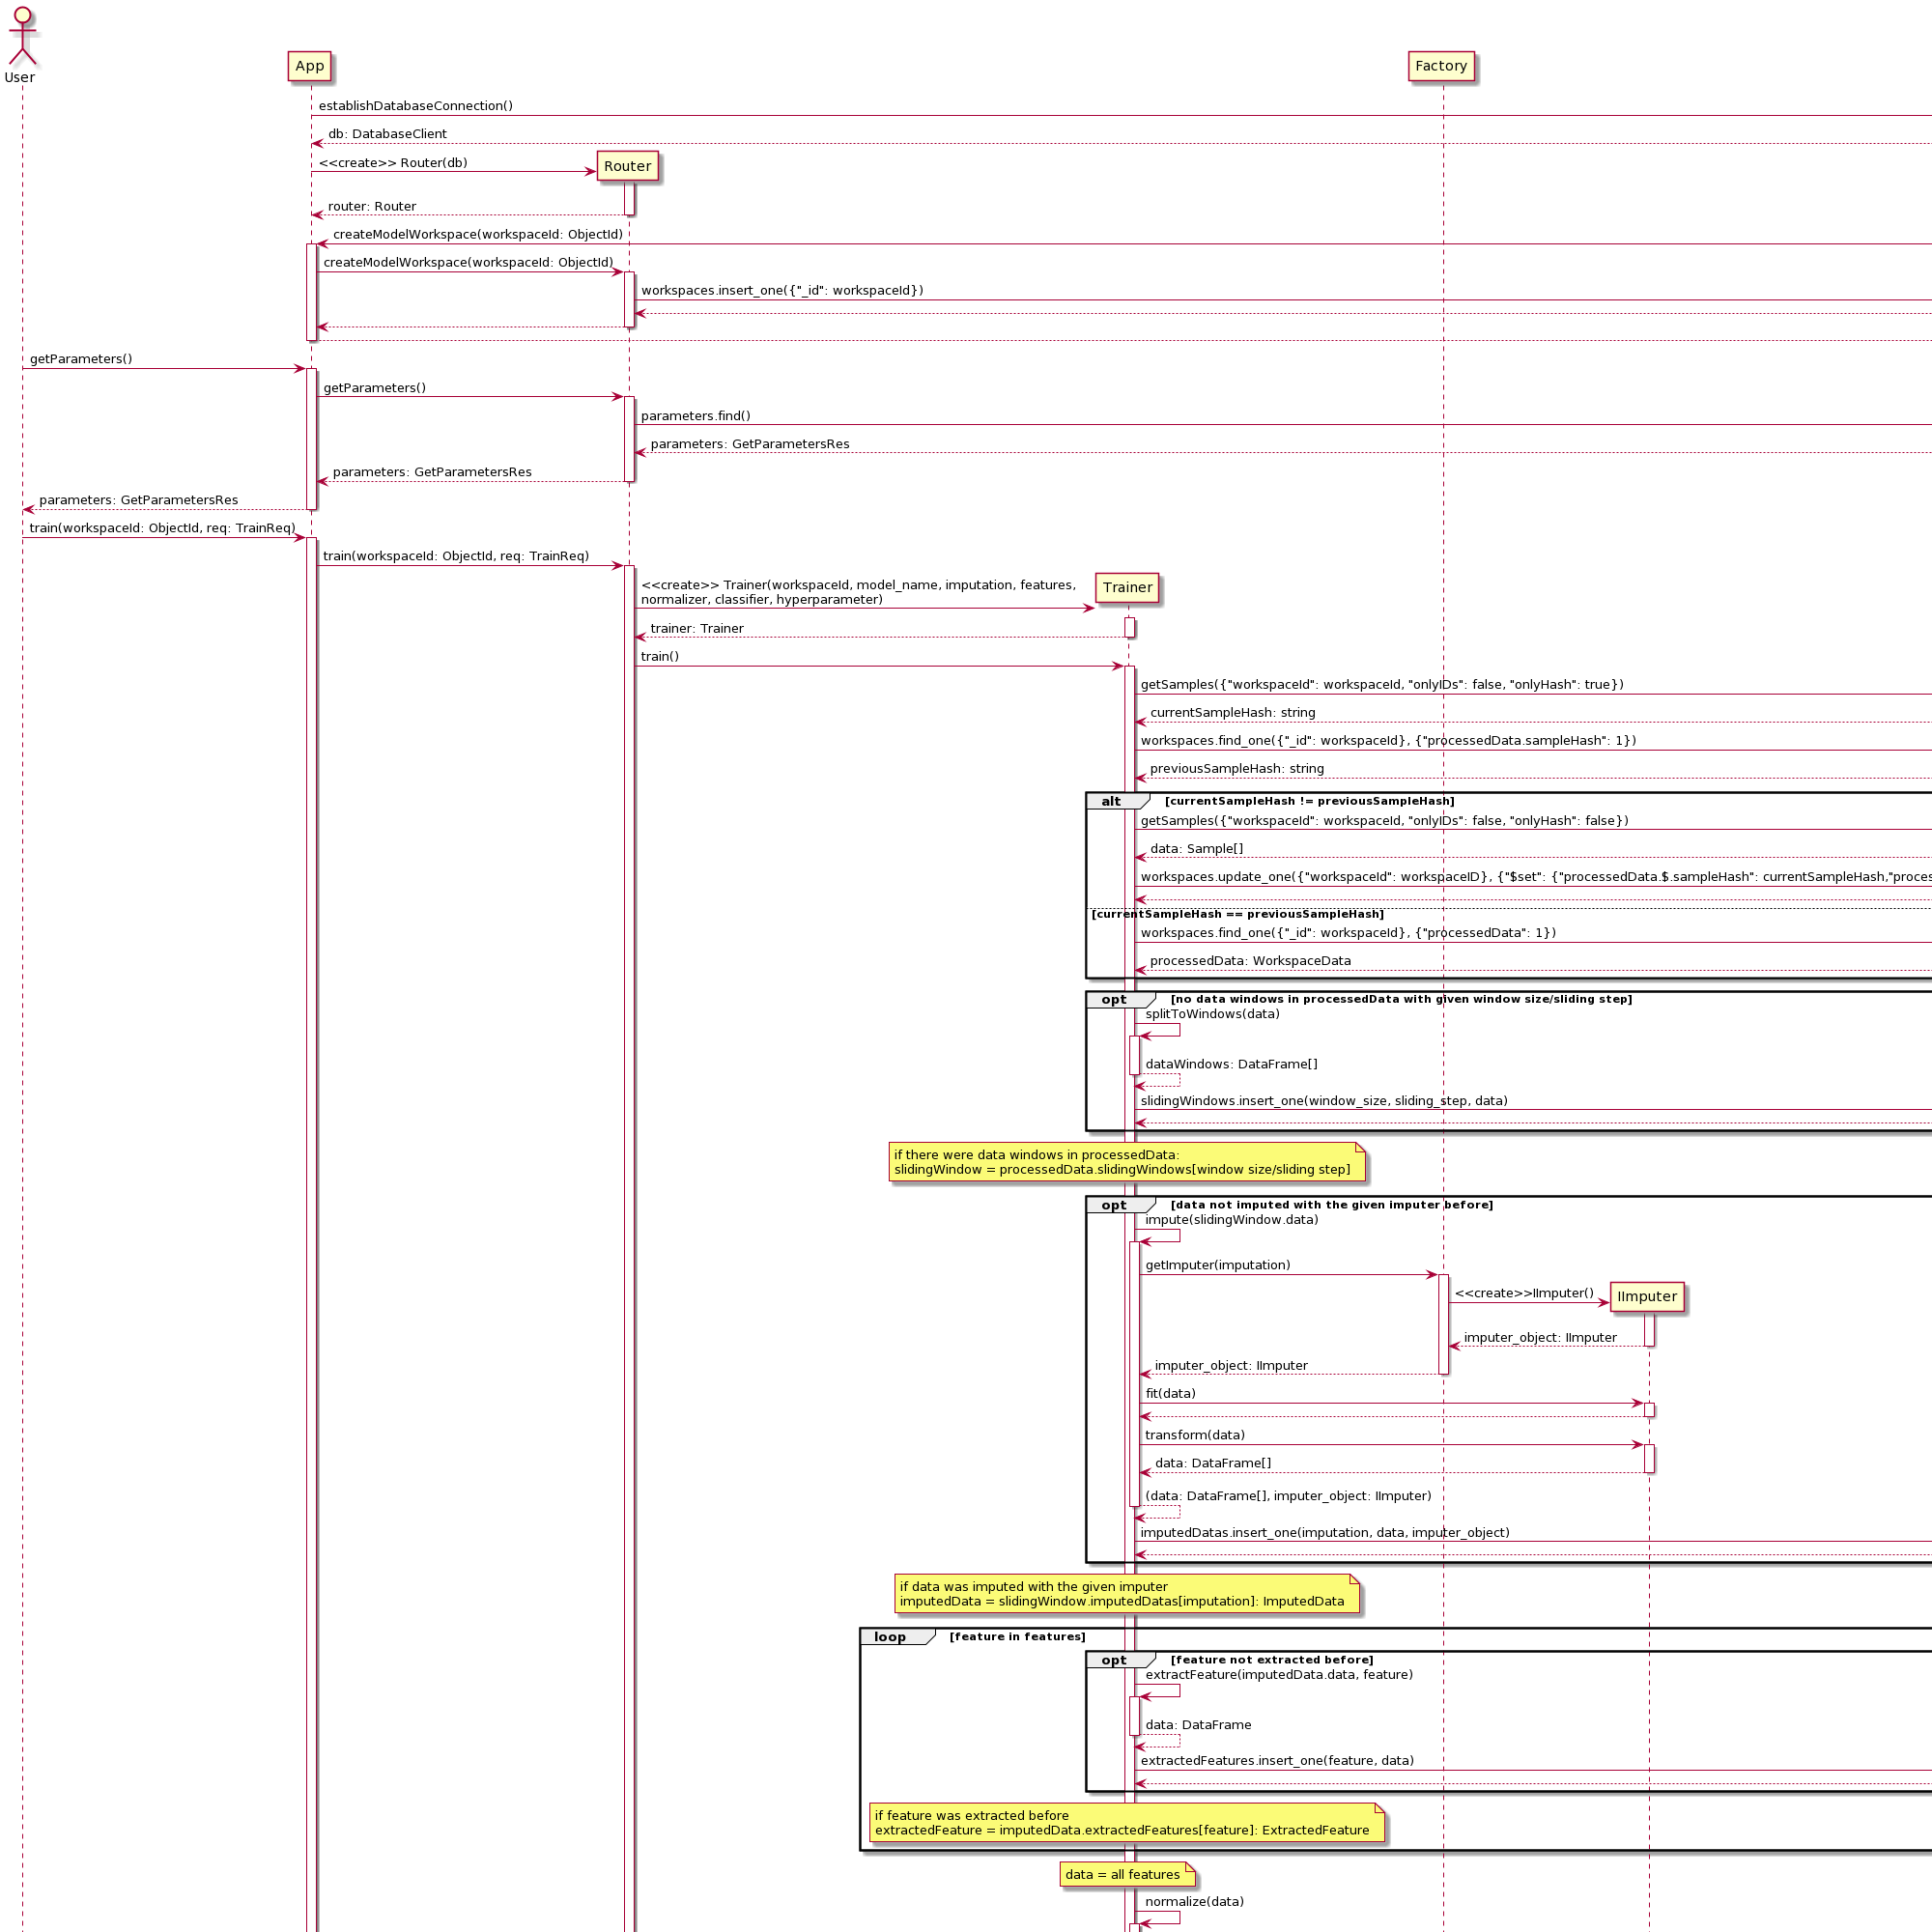
\includegraphics[width = 0.98\textwidth, height = 0.85\textheight]{figures/seq-training-a-model.png}}
    \caption{Model Training Sequence}
    \label{fig:seq-training-a-model}
\end{figure}


\subsubsection{Prediction}
In this sequence diagram, a user uses one of the trained models to classify his actions with his mobile. At first, the user gets all the IDs of the models and chooses the model which the user wants to use. The user then gets a prediction ID of this model, which is embedded in a QR code. When scanned, the mobile client requests the prediction configuration of this model, which returns the sensors to be used and their sampling rates. A new Predictor instance is created in the backend with the imputer, normalizer and classifier object of the model as well as the labels of the workspace. As long as the user submits data, the trainer does the needed imputation, feature extraction and normalization of the data. The classifier object then predicts the data. The trainer class counts the number of times the labels were predicted. When the getPrediction request is called, the label with the highest count of predictions is returned, and the counters are reset.
\begin{figure}[!htb]
    \centering
    \fbox{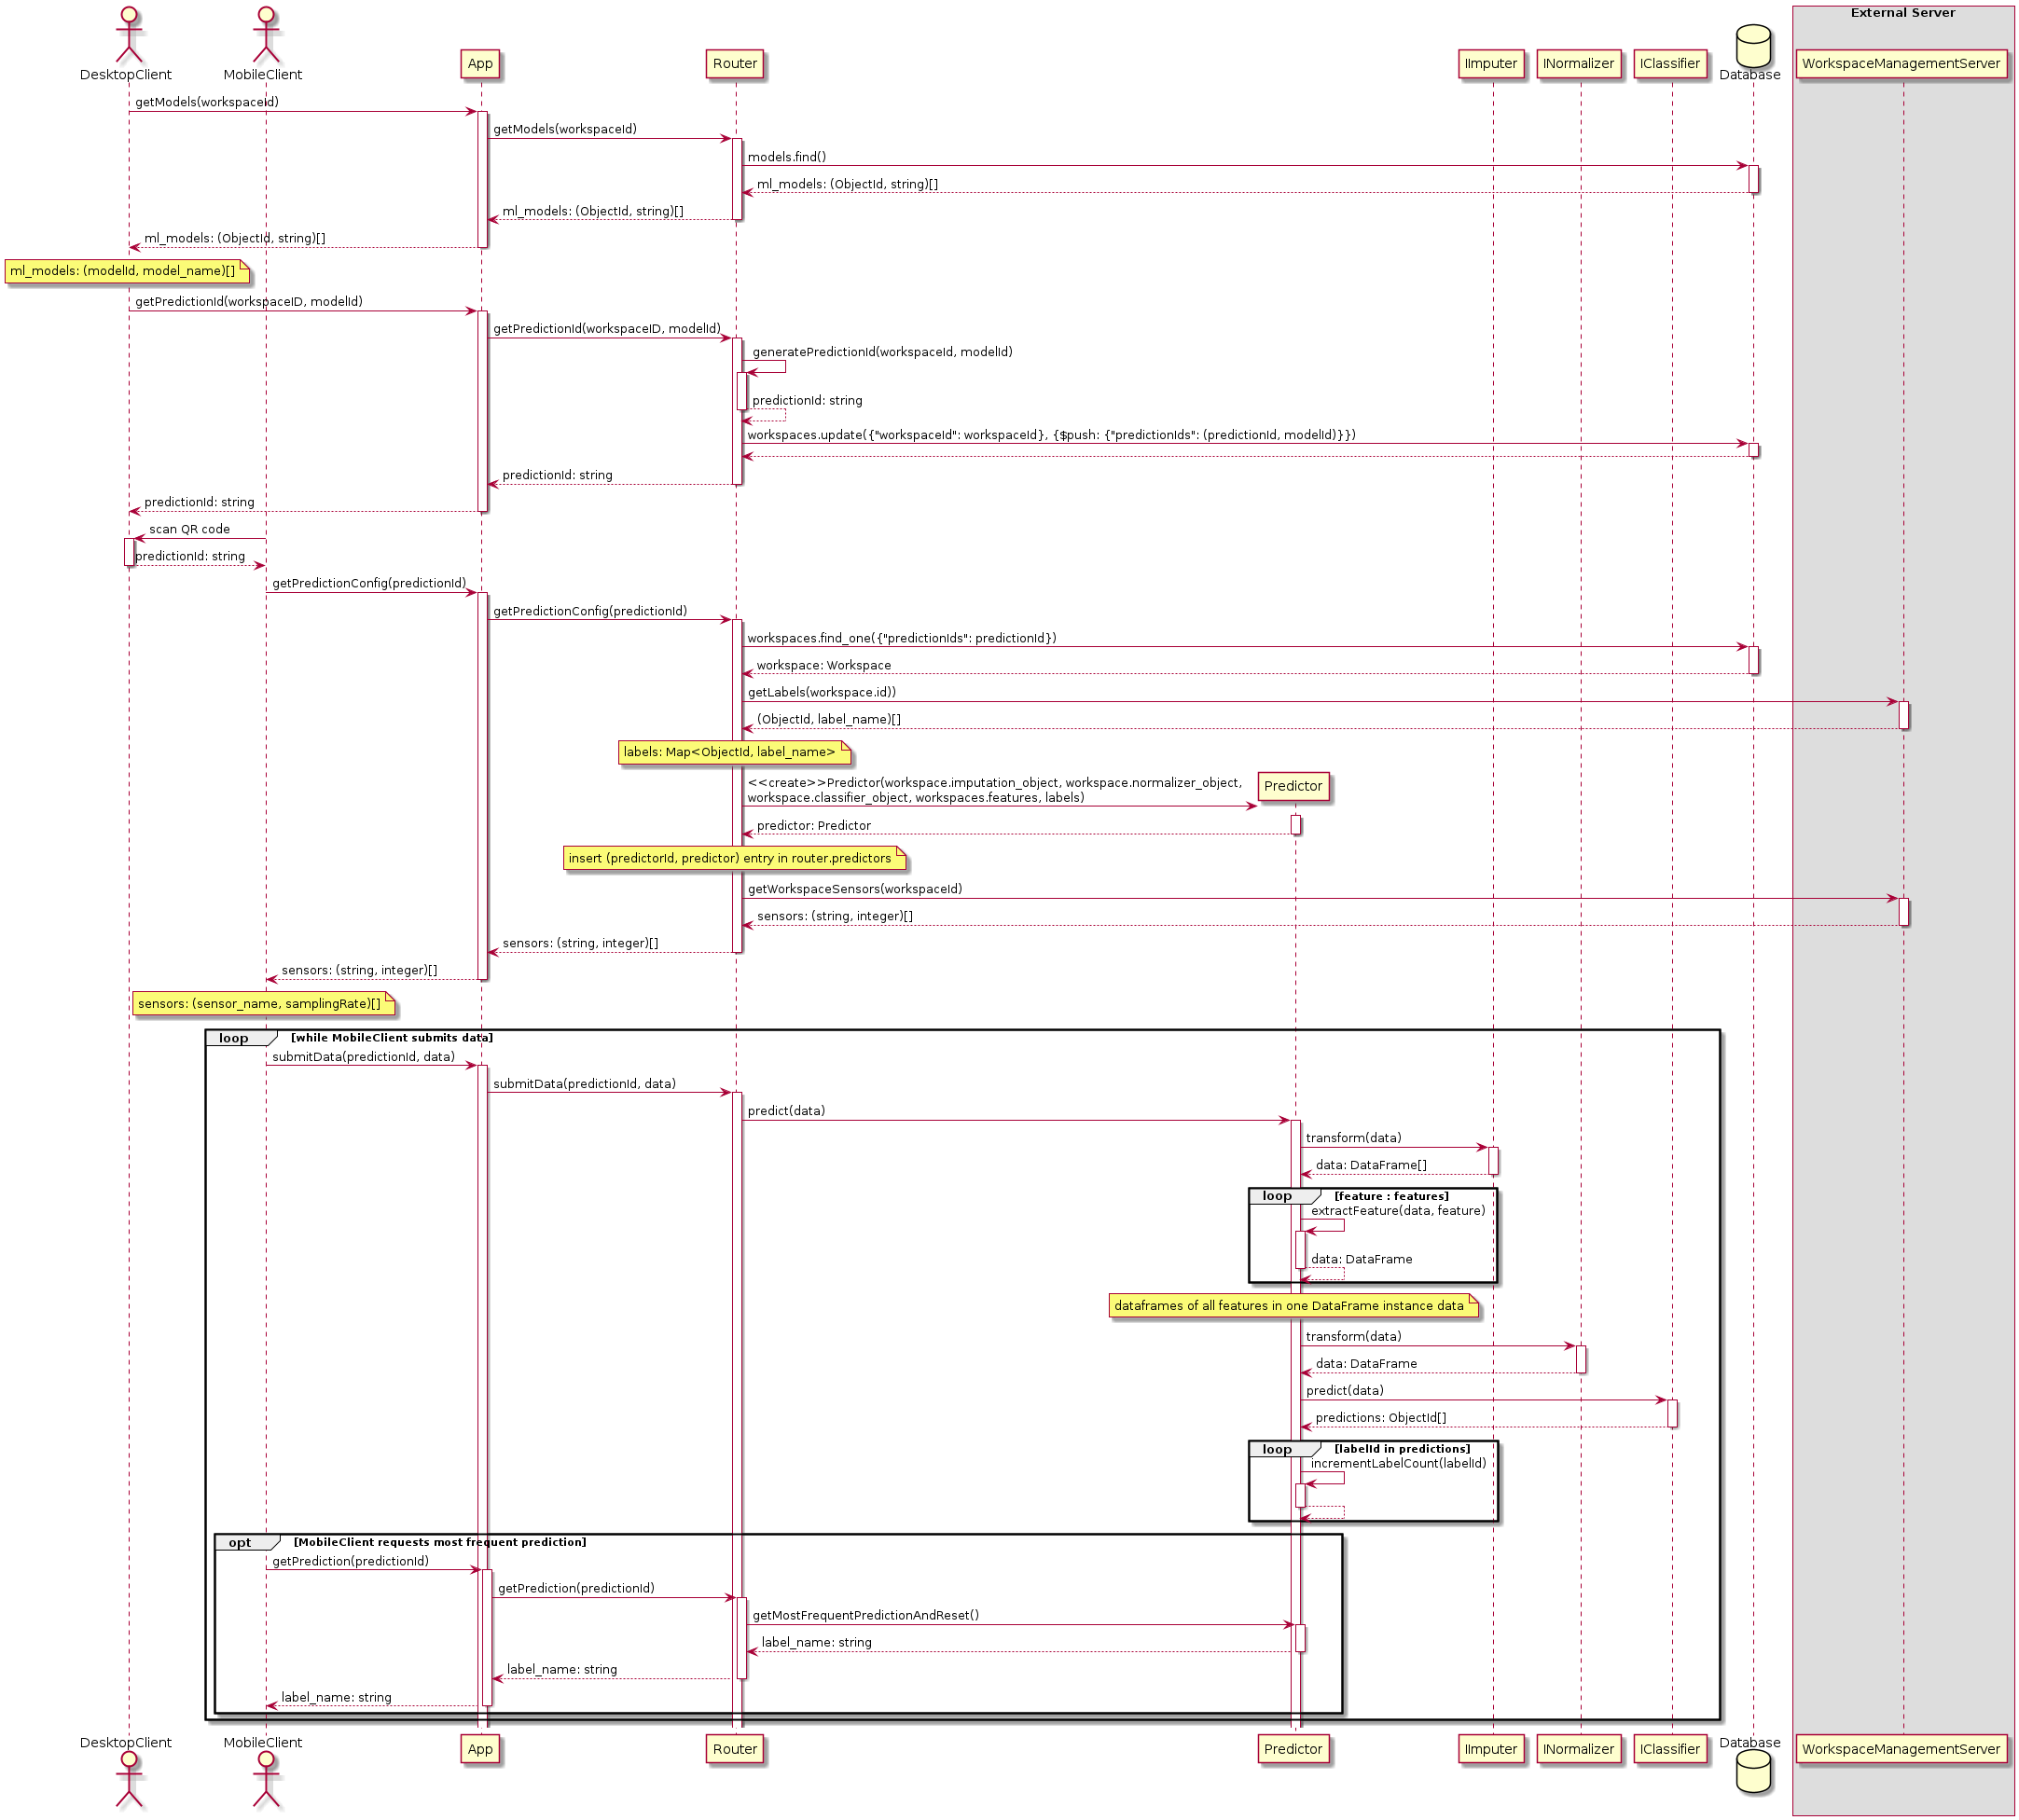
\includegraphics[width = 0.98\textwidth, height = 0.80\textheight]{figures/seq-predict.png}}
    \caption{Mobile Prediction Sequence}
    \label{fig:seq-predict}
\end{figure}

\textbf{explanation}